\chapter*{Реферат}
\addcontentsline{toc}{chapter}{Реферат} 

\begin{center}
    Общая характеристика диссертации
\end{center}

\begin{figure}
    \centering
    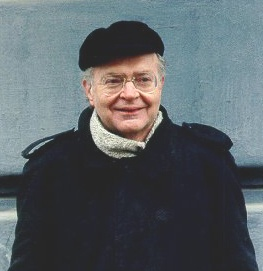
\includegraphics[width=0.6\linewidth]{images/knuth}
    \caption{Knuth}
    \label{fig:my_label2}
\end{figure}


\paragraph*{Актуальность.}

\paragraph*{Цель исследования.}
\paragraph*{Научные задачи.}

\paragraph*{Методы исследования.}

\paragraph*{Основные положения, выносимые на защиту.}
\begin{enumerate}
    \item \statementOneRU
    \item \statementTwoRU 
\end{enumerate}

\paragraph*{Научная новизна.}

\paragraph*{Теоретическая значимость.}
\paragraph*{Практическая значимость.}
\paragraph*{Достоверность.}
\paragraph*{Аппробация работы.}
\paragraph*{Личный вклад автора.}


\paragraph*{Объём и структура работы.}
Диссертация состоит из~введения,
\formbytotal{totalchapter}{глав}{ы}{}{},
заключения и
\formbytotal{totalappendix}{приложен}{ия}{ий}{}.
%% на случай ошибок оставляю исходный кусок на месте, закомментированным
%Полный объём диссертации составляет  \ref*{TotPages}~страницу
%с~\totalfigures{}~рисунками и~\totaltables{}~таблицами. Список литературы
%содержит \total{citenum}~наименований.
%
Полный объём диссертации составляет
\formbytotal{TotPages}{страниц}{у}{ы}{}, включая
\formbytotal{totalcount@figure}{рисун}{ок}{ка}{ков} и
\formbytotal{totalcount@table}{таблиц}{у}{ы}{}.
Список литературы содержит
\formbytotal{citenum}{наименован}{ие}{ия}{ий}.




\newpage
\section*{Основное содержание работы}

В Главе~\ref{ch:ch1}...

\section*{Публикации автора по теме диссертации}


Основные результаты по теме диссертации изложены в \theAllMyPapers~публикациях. 
Из них
%4 изданы в журналах, рекомендованных ВАК, 
\theScopusPapers~опубликовано в изданиях, индексируемых в базе цитирования Scopus. 
%Также имеется 1 свидетельство о государственной регистрации программ для ЭВМ.

В международных изданиях, индексируемых в базе данных Scopus:
\begin{refsection}[biblio/own.bib]
\nocite{*}
\printbibliography[
    keyword=scopus,
    %title={В международных изданиях, индексируемых в базе данных Scopus}, 
    %heading=subbibliography,
    heading=none,
    resetnumbers=true
]
\end{refsection}



В международных изданиях, индексируемых в базе данных Web of Science:
\begin{refsection}[biblio/own.bib]
\nocite{*}
\printbibliography[
    keyword=wos,
    %title={В международных изданиях, индексируемых в базе данных Web of Science}, 
    %heading=subbibliography,
    heading=none,
    resetnumbers=true
]
\end{refsection}
Список всех публикаций автора по теме диссертации:
\begin{refsection}[biblio/own.bib]
\nocite{*}
\printbibliography[
    keyword=own,
    %title={Список всех публикаций автора по теме диссертации}, 
    %heading=subbibliography,
    heading=none,
    resetnumbers=true
]
\end{refsection}
